\documentclass[a4paper,12pt]{article}
\usepackage[a4paper,top=2.0cm, bottom=1.5cm, left=1.5cm, right=1.5cm]{geometry}

\usepackage[T2A]{fontenc}			
\usepackage[utf8]{inputenc}		
\usepackage[english,russian]{babel}	
\usepackage{amsmath,amsfonts,amssymb,amsthm,mathtools} 
\usepackage{wasysym}
\usepackage{graphicx}
\usepackage{wrapfig}
\usepackage{amsmath}
\usepackage{ mathrsfs }
\DeclareMathOperator*{\argmax}{argmax}
\DeclareMathOperator*{\argmin}{argmin}
\DeclareGraphicsExtensions{.pdf, .png, .jpg}
\graphicspath{{}}


\begin{document}
	\section{Введение}
		В последние годы, методы машинного обучения позволяют добиваться успехов в задачах рекомендации, однако задачи требующие подбора группы объектов совместимых между собой все еще представляют серьезную проблему. Основным препятствием является неизвестный характер зависимости между объектами в таких группах. В работе исследуется необходимость и способы построения аппроксимации этой зависимости для прикладной задачи рекомендации наборов одежды называемых <<образами>>.
		В частности, в отличие от ранее представленных работ, рассматриваются методы решения задачи рекомендации более одного элемента одежды, дополняющих заданный <<образ>>. Предлагается рассмотреть двухшаговый подход к приближенному решению дискретной оптимизационной задачи,  превосходящий по скорости ранее представленные и сравнить его качество с методом жадного перебора -- лучшим вычислимым за ограниченное время. Для аппроксимации зависимости между элементами образа предлагается использовать графовые нейронные сети (GNN) \cite{scarselli2008graph}.
		
		...
		
			
	\section{Постановка задачи}
		\subsection{Основные понятия}
			Основная единица данных, рассматривающаяся в работе -- элемент одежды, далее будем называть его \textit{объектом} или \textit{элементом}, множество всех рассматриваемых объектов -- $\mathcal{X}$. 
			
			Каждый объект $X\in\mathcal{X}$ представим как пару $X = (I, T)$ соответственно изображения объекта (может отсутствовать) и его текстового описания(может быть пустым). Пусть $\mathcal{I}$ -- множество изображений объектов.
			
			Некоторое подмножество $O = \{X_i\}_{i=1}^k\subset \mathcal{X}$ множества всех элементов будем называть \textit{образом}, если
			\begin{enumerate}
				\item $O\neq\{\O\}$
				\item $|O| \leqslant K$
			\end{enumerate}
		    где $K$ -- определяемая задачей константа. 
			Множество всех образов обозначим $\mathcal{O}$.
		    
			Для элементов и образов будем рассматривать \textit{функции близости}
				$$S_X:~\mathcal{X}\times \mathcal{X}\longrightarrow [-1,1], ~~\forall X\in\mathcal{X}~S_X(X,X) = 1$$
				$$S_O:~\mathcal{O}\times \mathcal{O}\longrightarrow [-1,1], ~~\forall O\in\mathcal{O}~S_O(O,O) = 1$$
			Такой функцией может выступать например косинусное сходство в некотором латентном пространстве.
				
			Для оценки образов введем функцию \textit{оценки} или \textit{совместимости} его элементов: 
			$$\mathcal{S}:~2^\mathcal{X}\longrightarrow [0,1]$$
			 причем выполнено следующее:
			$$\forall O \in \mathcal{O}:~\mathcal{S}(O) > 0$$
			$$\forall O' \in 2^\mathcal{X} \setminus \mathcal{O}: \mathcal{S}(O') =0$$
			\textit{Совместимостью} или \textit{оценкой совместимости} образа $O$ будем называть результат применения функции совместимости к этому образу $\mathcal{S}(O)$
			
		\subsection{Описание рассматриваемых задач}
			\subsubsection{Оценка образа}
				Выше введена функция $\mathcal{S}$, ассоциирующая с каждым образом его оценку совместимости, однако вид такой функции неизвестен. Задача оценки образа -- это классическая задача регрессии:\\
				\begin{itemize}
					\item \textbf{Дано:}\\
						$\{O_1\dots O_n\}\subset \mathcal{O}$\\
						$\{\mathcal{S}(O_1)\dots\mathcal{S}(O_n)\}$
					\item \textbf{Требуется:}\\
					Найти наилучшую в некотором смысле аппроксимацию функции $\mathcal{S}$ функциями заданного класса, т.е. решить задачу оптимизации:\\
					$$\hat{\mathcal{S}}= \argmin_{S}\left[\frac{1}{N} \sum\limits_{i=1}^N\mathcal{L}(\mathcal{S}(O_i), S(O_i))\right]$$
					где $\mathcal{L}(\cdot, \cdot)$ некоторая метрика, например евклидова
				\end{itemize}
			
				\subsubsection{Описание образа (скорее всего уберу)}
				Задача описания образа есть задача построения наилучшего текстового описания для данного образа по изображениям его элементов. Полагая функцию оценки известной получаем следующую формальную постановку:\\
				\begin{itemize}
					\item \textbf{Дано:}\\
					$\{X_i\} = O_n, ~|O_n| = n$ --- образ, где $X_i = (I_i, \O),~I_i\in\mathcal{I},~i=\overline{1, n}$ --- его элементы с пустым текстовым описанием. \\
					$O_n(T) = \{X_i(T) = (I_i, T)\}_{i=1}^n$ для некоторого общего описания $T$\\
					\item \textbf{Требуется:}\\
					Найти оценку $\hat{T}$ общего для всех элементов описания $T$, максимизирующую значение функции оценки $\mathcal{S}(O_n)$, т.е.: \\
					$$\hat{T}= \argmax_{T}\mathcal{S}(O_n(T))$$
				\end{itemize}
				Стоит заметить, что в данном случае задача генеративная --- лучшее описание находится, из решения задачи максимизации функции оценки, а не просто выбирается из заранее заданного конечного множества.
				
			
			\subsubsection{Дополнение (восстановление) образа}
				Для решения задачи восстановления образа необходимо знать функцию совместимости или ее аппроксимацию. Предполагая ее известной, получаем следующую постановку:
				\begin{itemize}
					\item \textbf{Дано:}\\
					$O_n\in\mathcal{O}, ~|O| = n$ \\
					$k \in \mathbb{N}, ~k> n$ --- количество недостающих элементов\\
					$\{\hat{T_i}\}_{i=1}^k$ --- текстовые представления недостающих элементов, возможно пустые. В случае если предлагается только текстовое описание всего образа $T$, оно используется в качестве описания каждого элемента, т.е. $\forall i \in \overline{1,k}: ~T_i = T$.
					
					\item \textbf{Требуется:}\\
					Найти наилучшее в смысле максимизации функции оценки дополнение образа $O_n$ до $O_k\in\mathcal{O}, |O_k|=k$, т.е. решить следующую задачу:
					$$\{\hat{X_i}\}_{i=1}^k= \argmax_{\{X_i\}_{i=1}^k\in \mathcal{X}^k} \left[\alpha \cdot \mathcal{S}\left(O_n\cup\{X_i\}_{i=1}^k\right) + (1-\alpha) \cdot \sum\limits_{i=1}^k S_X((I_i, T_i), (I_i, \hat{T_i}))\cdot\mathbb{I}\{\hat{T_i}\neq\O\}  \right]$$				
					здесь $X_i = (I_i, T_i)$, $\alpha\in[0,1]$. Второе слагаемое отвечает за соответствие предсказанного элемента предъявленному текстовому представлению и равно нулю, если представление пусто. Задача, в отличие от предыдущей, дискриминативная и  может быть решена точно полным перебором всех объектов из $\mathcal{X}$.
				\end{itemize}
			
			\subsubsection{Генерация образа (скорее всего уберу)}
				Задача генерации состоит в выборе образа произвольного размера, наиболее подходящего к предоставленному текстовому описанию. В терминах введенных выше получаем:
			
				\begin{itemize}
					\item \textbf{Дано:}\\
					$T$ --- текстовое описание образа.
					
					\item \textbf{Требуется:}\\
					Найти наилучший в смысле максимизации функции оценки образ $O\in\mathcal{O}$ элементы которого наилучшим образом соответствуют предложенному описанию $T$, т.е.:
					$$ \hat{O} = \argmax_{k,O = \{X_i\}_{i=1}^{k},  O\in\mathcal{O}} \left[\alpha \cdot \mathcal{S}(O) + (1-\alpha) \cdot \sum\limits_{i=1}^{k} S_X((I_i, T_i), (I_i, T))\cdot\mathbb{I}\{\hat{T}\neq\O\}  \right]$$				
					здесь $X_i = (I_i, T_i)$, $\alpha\in[0,1]$. 
					Стоит заметить, что если зафиксировать $k=1$, получаем обычную задачу поиска наиболее подходящего под описание элемента в коллекции. Учитывая то, что множество образов определено множеством элементов и определением образа, задача генерации образа также является дискриминативной и состоит в переборе всех возможных образов.
				\end{itemize}
			
		\subsection{Обзор литературы}
			\subsubsection{Подходы к построению функций близости}
				При рассмотрении проблемы построения достаточно информативной функции от образов встает вопрос о том какие особенности структуры исходных данных могут быть полезны и на чем можно основывать выбор архитектуры. 
				
				Поскольку образ состоит из переменного числа первоначально независимых элементов, естественно перед рассмотрением образа независимо получать некоторое представление каждого его элемента. Кроме того, понятно, что операции с элементами внутри образа должны быть эквивариантны к перестановке элементов, поскольку на них не возникает естественного порядка. Развивая эту идею, можно сказать что каждому элементу присущ некоторый набор признаков, часть из которых может существенно влиять на совместимость, а значит декомпозиция элементов на признаки, моделирование их взаимосвязей а также взаимосвязей элементов между собой может помочь в построении оценки всего образа. 
				
				Подобным образом декомпозированная на разные масштабы задача может быть представлена например в виде графа, а значит одним из способов решения будут графовые нейронные сети. Такой подход в контексте оценки и подбора образов рассматривают в частности в статьях <<Fashion Retrieval via Graph Reasoning Networks on a Similarity
				Pyramid>> \cite{https://doi.org/10.48550/arXiv.1908.11754} и <<Hierarchical Fashion Graph Network for Personalized Outfit
				Recommendation>> \cite{https://doi.org/10.48550/arXiv.2005.12566}. \\
				
				В \cite{https://doi.org/10.48550/arXiv.1908.11754} авторы предлагают GRNet – модель для определения похожести элементов, которая обрабатывает несколько представлений изображения каждого элемента (текстовые описания в статье не рассматривается) в разном масштабе. Т.е. авторы использует еще один промежуточный уровень -- масштаб -- для построение латентного представления каждого элемента. 
				
				В предложенной модели для каждого элемента сначала с помощью GoogLeNet \cite{https://doi.org/10.48550/arXiv.1409.4842} создаются несколько представлений как раз и называемых масштабами, далее несколько вырезанных частей каждого из полученных представлений называются признаками. Считаются локальные векторы близости между соответствующими признаками в соответствующих масштабах, в конце осуществляется message passing \cite{https://doi.org/10.48550/arXiv.1704.01212} по полному графу, вершинами которого являются вычисленные векторы. Таким образом, вместо рассмотрения единого векторного представления, каждый элемент, пользуясь предполагаемой симметрией задачи, декомпозируют на несколько масштабов, а каждый масштаб на несколько признаков и моделируют их взаимодействие.
				
				Оставим за пределами нашего рассмотрения подробности процесса получения признаков, тогда пусть для элементов $X, Y\in \mathcal{X}$,  $\{x_l^i \in \mathbb{R}^{C\times 1}\}$ и $\{y_l^i \in \mathbb{R}^{C\times 1}\}$ векторные представления $i$-го локального признака в $l$ масштабе. Для каждого масштаба $l$ и номеров признаков $i$ и $j$ вектор локальной близости --- $s_l^{ij}$:
				$$s_l^{ij} = \frac{P|x_l^i-y_l^j|^2}{\|P|x_l^i-y_l^j|^2\|_2}$$
				где $P$ -- так называемая проекционная матрица с обучаемыми весами.\\
				Из этих векторов составляется граф, называемый авторами пирамидой. Далее для каждой пары вершин $s_{l_1}^{ij}$ и $s_{l_2}^{mn}$ определяется скаляный вес $w_p^{l_1ijl_2mn}$:
				$$w_p^{l_1ijl_2mn} = \frac{\exp((\mathbf{T}_{out}s_{l_1}^{ij})^\intercal(\mathbf{T}_{in}s_{l_2}^{mn}))}{\sum\limits_{l,p,q}\exp((\mathbf{T}_{out}s_{l_1}^{ij})^\intercal(\mathbf{T}_{in}s_{l}^{pq}))}$$ 
				где $\mathbf{T}_{in}, \mathbf{T}_{out}$ -- обучаемые матрицы.
				Тогда для $l_1=l_2$ это веса внутри одного масштаба, а для $l_1\neq l_2$ -- между разными, что позволяет им "сообщаться". Таким образом мы определили граф близости $G = (\mathbb{N},\mathbb{E})$, где $\mathbb{N} = \{s_l^{ij}\}$ а $\mathbb{E} = \{w_p^{l_1ijl_2mn}\}$.\\
				Далее вектора в каждой вершине обновляются по следующему правилу:
				$$\widehat{s}_{l_1}^{ij} =ReLU\left(\mathbf{W} \sum\limits_{l_2,m,n}w_p^{l_1ijl_2mn}s_{l_2}^{mn}\right)$$
				где $\mathbf{W}$ -- еще одна обучаемая матрица параметров. Итоговая оценка близости получается в дополнительной вершине графа, которая предварительно инициализируется некоторой простой функцией $s_g$:
				$$s_g = S_g(A(X), A(Y))$$
				где $A(.)$ --- например average pooling или max pooling по всем признакам во всех масштабах, а $S_g$ ---  например косинусное сходство.\\
				
				В \cite{https://doi.org/10.48550/arXiv.2005.12566} авторы используют схожий подход к декомпозиции для задачи рекомендации образов. Рассматривается иерархическая структура из трех уровней --- уровня элементов, уровня образов уровня пользователей. Для рассматриваемых пользователей, образов и элементов всех этих образов строится соответствующих трехуровневый граф с ребрами направленными с уровня элементов в уровень образов и из уровня образов в уровень пользователей. Далее, начиная с нижнего уровня, с помощью фактически чуть упрощенного подхода графовых сверточных сетей \cite{https://doi.org/10.48550/arXiv.1609.02907}, латентные представления элементов последовательно агрегируются в латентные представления на уровне образов и на уровне пользователей, которые непосредственно используются для рекомендации путем выбора для пользователя с представлением $u^*$ образа $\hat{O}$ по правилу $$\hat{O} = \argmax_{O\in \mathcal{O}}f(O)^\intercal u^*$$
				где $f(O)$ --- представление образа, полученное при подсчете в том же графе.
				
			\subsubsection{Восстановление, генерация и оценка образов}
				В задачах оценки, генерации и рекомендации образов, как и во многих других, хорошо показывают себя специальным образом обученные трансформерные \cite{https://doi.org/10.48550/arXiv.1706.03762} архитектуры. Заметим, что в силу отсутствия порядка на элементах и их признаках трансформер без позиционного кодирования \cite{https://doi.org/10.48550/arXiv.1706.03762} фактически эквивалентен graph attention network \cite{
				https://doi.org/10.48550/arXiv.1710.10903} с несколькими LayerNorm \cite{
				https://doi.org/10.48550/arXiv.1607.06450} и линейными слоями. Таким образом, при использовании этой архитектуры мы также неявно учитываем рассмотренную выше симметрию данных. 
				Варианты применение трансформеров для задач связанных с образами рассмотрены в частности в статьях \cite{https://doi.org/10.48550/arXiv.2303.02483} и \cite{https://doi.org/10.48550/arXiv.2204.04812}.\\
				
				В \cite{https://doi.org/10.48550/arXiv.2204.04812} авторы предлагают использовать архитектуру трансформера для обучения представления образа целиком. Полученное представление используется для оценки совместимости образа и восстановления образа с пропущенными элементами. В качестве токенов в трансформер подаются латентные представления элементов, т.е. фактически обрабатывается полный граф из всех элементов образа. Помимо изображений элементов, авторы также используют их текстовое описание и одновременно тренируют 2 энкодера для текстового и графического представления каждого объекта. Для задачи восстановления/рекомендации в модель также подается дополнительный токен, инициализированный случайный образом, после прохождения через модель агрегирующий в себе информацию из всех остальных и использующийся в итоге непосредственно для выбора ближайшего в смысле максимизации скалярного произведения дополняющего образ элемента.
				
				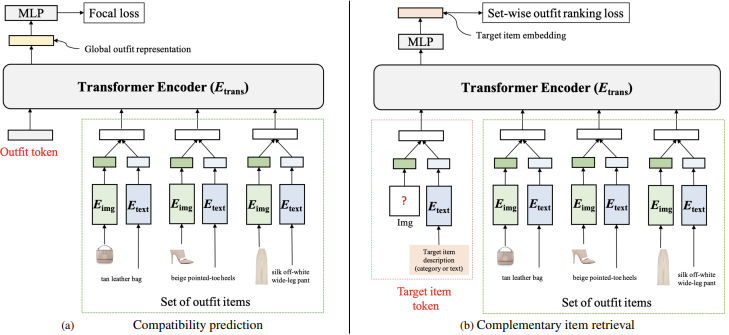
\includegraphics[scale = 0.8]{OutfitTransfromer intro.png}
				
								
				(перерисовать картинку из статьи??)\\
				
				Предложенную модель обучают сначала для оценки совместимости образа, а затем заменяют последние линейные слои и дообучают получать представление образа для подбора подходящих элементов на основании полученного представления и текстового описания нового элемента. Из этого можно заключить, что учет внутренней структуры оказывается полезным и для оценки образа целиком, и для восстановления отдельных его частей, причем для разных задач возможно использовать одни и те же латентные представления элементов. \\
				
				Идею с общими внутренними представлениями для разных задач развивают авторы \cite{https://doi.org/10.48550/arXiv.2303.02483}. В статье рассматривается вопрос обучения мультимодального трансформера одновременно на несколько задач связанных с образами. 
				
				\begin{wrapfigure}{l}{0.5\linewidth}
					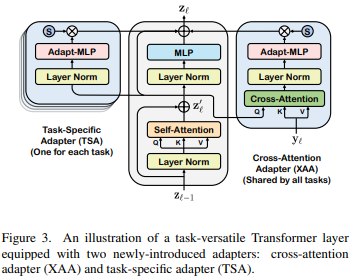
\includegraphics[scale = 1.0]{FAME-ViL_acrhitecture.png}
				\end{wrapfigure}
				
				Основой архитектуры предложенной модели выступает предтренированный CLIP \cite{https://doi.org/10.48550/arXiv.2103.00020}. Для того, чтобы приспособить модель к выполнению различных задач рекомендации, распознавания и оценки образов авторы предлагают 2 вида адаптеров: TSA -- Task-Specific Adapter для обучения специфическим для каждой задачи особенностям и XAA -- Cross-Attention Adapter для обеспечения возможности взаимодействиями между различными модальностями, общий для всех задач. Для TSA предлагается ввести дополнительные линейные слои (AdaptMLP) после каждого self-attention блока параллельно с основными:
				$$z_l^{tsa}=s \cdot AdaptMLP(LN(z'_l))$$
				где $s$ -- Обучаемый множитель.\\
				В XAA используется дополнительный Multi-Head Cross Attention (MHXA) с группой линейных слоев после него:
				$$z_l^{xaa} = s\cdot AdaptMLP(LN(MHXA(z_l',y_l)))$$
				где $y_l$ выход self-attention слоя части сети для другой модальности.\\
				Далее полученные $z_l^{tsa}$ и $z_l^{xaa}$ аггрегируются с обычным выходом следующим образом:
				$$z_l = MLP(LN(z_l')) + z_l'+z_l^{tsa}+\epsilon\cdot z_l^{xaa},~\epsilon\in\{0,1\}$$
				$\epsilon$ -- барьерный множитель включающий или выключающий определенный адаптер для определенной задачи. 
				
				Рассматриваемая архитектура обучается на разные задачи в трех режимах Contrastive, Fusion и Generative с различными используемыми адаптерами и функциями потерь. 
				
				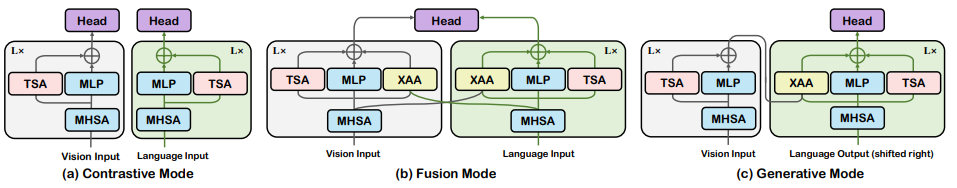
\includegraphics[scale = 0.7]{FAME-ViL_modes.png}
				
				\begin{itemize}
					\item[]\textbf{Contrastive mode:}\\
					Этот режим используется для кросс-модальных рекомендаций (XMR) --- задачи выбора наиболее подходящего элемента по текстовому описанию и выбора наиболее подходящего описания элемента на изображении среди данных. Все XAA блоки отключены. Обучение производится на выборках элементов $\mathcal{X} \supseteq (\textbf{I}, \textbf{T}) = \{(I_1, T_1), \dots, (I_B, T_B)\}$, сначала части сети для соответствующей модальности по отдельности применяются к элементам каждой пары, формируя 2 итоговых унимодальных представления, а потом с помощью контрастной функции потерь \cite{https://doi.org/10.48550/arXiv.2004.11362} производится максимизация схожести получившихся унимодальных представлений.
					$$\mathcal{L}_{XMR} = \frac{1}{2} [\mathcal{L}_{InfoNCE}(\mathbf{T}, \mathbf{I}) + \mathcal{L}_{InfoNCE}(\mathbf{I}, \mathbf{T})]$$
					$$\mathcal{L}_{InfoNCE} = -\frac{1}{B}\sum\limits_{i=1}^{B}\log\frac{\exp(s(X_i, Y_i)/\tau)}{\sum_{j=1}^B\exp(s(X_i, Y_j)/\tau)}$$
					где $\tau$ -- обучаемая (???) температура. $s$ -- симметричная функция схожести $s(I_i, T_j) = f_\theta^{[c]}(I_i)^T\cdot f_\theta^{[c]}(T_j)$, где $f_\theta^{[c]}$ -- собственно нейросеть.
					\item[]\textbf{Fusion mode:}\\
					Используется для субкатегориального распознавания (SCR)и направляемых текстом рекомендаций (TGIR). И XAA, и TSA блоки включены. \\
					Задача SCR -- предсказание подкатегории для данного товара, основываясь на тексте и картинке. Исходя из специфики задачи, к выходу сети дополнительно добавляется классификатор, cross-entropy-loss которого и минимизируется:
					$$\mathcal{L}_{SCR} = -\mathbb{E}_{(I,T)\sim D}\log P\left(f_\theta^{[f]}(I, T)\right)$$
					Для TGIR --нахождения элементов похожих по изображению на данный и соответствующих текстовому описанию -- подход немного другой, поскольку необходимо получить представления отдельно для исходной картинки с текстовым описанием и целевой картинки, поэтому для $(\mathbf{I^r}, \mathbf{T})$ соответственно исходных картинок и текстовых запросов сеть запускается в $fusion$ режиме, а для целевых изображений $I^t$ в $contrastive$ режиме. Далее считается контрастная функция потерь вида
					$$\mathcal{L}_{TGIR} = \mathcal{L}_{InfoNCE}((I^r,T), I^t)$$
					
					\item[]\textbf{Generative mode:}\\
					Используется, например, для генерации описания к изображениям элементов. TSA блоки включены в обеих модальностях, XAA -- только image-to-text. Причем часть обрабатывающая входное изображение используется как энкодер, а вторая -- как декодер в авторегрессионном режиме.
				\end{itemize}
			
		\section{Теоретическая часть}
				Отличительной особенностью рассмотренных выше подходов является, попытка в том или ином виде моделировать взаимодействие многие ко многим в полном графе из частей внутренней структуры образов (элементов или признаков). Для моделирования взаимодействия между составными частями объекта или образа, нужно, для начала, получить некоторое их векторное представление. 
				
				В работе не будем сравнивать между собой способы векторизовать текстовые и графические представления и заранее их зафиксируем. Более того, сконцентрируемся на представлении образа как множества элементов без внутренней структуры и оставим вопрос разбиения объектов на признаки и рассмотрения их взаимодействия за рамками данной работы.
								
				Для получения представлений текстового и графического описания каждого элемента будем использовать предобученную модель <<Outfit Transformer>>\cite{https://doi.org/10.48550/arXiv.2204.04812}. Под множеством объектов $\mathcal{X}$ далее будем подразумевать множество их векторных представлений $\mathcal{X}\subset \mathbb{R}^d$
				
				Будем рассматривать задачу дополнения образа. Для ее решения, как было сказано, необходимо знать функцию совместимости. Оставим восстановление этой функции за рамками текущей работы и снова будем пользоваться ранее предложенным решением -- предобученной моделью из \cite{https://doi.org/10.48550/arXiv.2204.04812}, для действия этой модели на образ будем использовать обозначение введенное выше для функции оценки --- $\mathcal{S}(\cdot)$. 
				$\mathcal{S}(\cdot)$ --- ограниченная непрерывно дифференцируемая функция своих аргументов, причем норма ее градиента также ограничена. 
				
				Далее нас будет интересовать исключительно случай пустого описания недостающих элементов. Учитывая постановку определенную ранее, получаем задачу следующего вида:
				\begin{itemize}
					\item \textbf{Дано:}\\
					$O_n\in\mathcal{O}, ~|O| = n$ --- исходный образ \\
					$k \in \mathbb{N}, ~k$ --- количество недостающих элементов\\					
					\item \textbf{Задача:}\\
					$$\{\hat{X_i}\}_{i=1}^k= \argmax_{\{X_i\}_{i=1}^k\subset\mathcal{X}} \mathcal{S}\left(O_n\cup\{X_i\}_{i=1}^k\right)$$
				\end{itemize}
				Для $k > 1$ и большого количества доступных элементов решение задачи полным перебором  становится вычислительно невозможным (сложность алгоритма полного перебора $|\mathcal{X}|^k$), поэтому необходимо рассмотреть возможные способы приближенного решения. 
				
			\subsection{Дискретный подход}\label{discrete}
			Заметим, что математически задача выбора $k$ наиболее подходящих к образу элементов может быть переформулирована как задача поиска наилучшего пути длины $k$ в полном графе, множество вершин которого есть 
			$$\mathcal{X}\setminus O_n \cup \{X_{init}\},$$ где $X_{init}$ -- дополнительная начальная вершина. Для некоторого пути $X_{init}, X_1, X_2\dots X_j$ можно рассчитать его <<\textit{оценку}>> как оценку образа $O_n\cup\{X_1\dots X_j\}$ тогда понятно, что поиск пути с максимальной оценкой эквивалентен решению поставленной выше задачи дополнения образа. Такой подход требует подсчета оценки текущего пути на каждом шаге, а значит чтобы улучшить асимптотику и получить практически вычислимый алгоритм, необходимо использовать приближенное решение задачи поиска в графе.
			
			В качестве бейзлайна будем рассматривать два следующих жадных алгоритма:
			\begin{enumerate}
				\item <<Одношаговый>> $|\mathcal{X}|$ вызовов функции оценки
				\begin{itemize}
					\item Подсчет $\mathcal{S}(O_n \cup X)$ для всех элементов $X\in \mathcal{X}$
					\item Выбор элементов $X_i,~i=\overline{1,k}$ соответствующих k максимальным значениям $\mathcal{S}(O_n \cup X)$
				\end{itemize}
				\item <<Многошаговый>> $k\cdot|\mathcal{X}|$ вызовов функции оценки
				\begin{itemize}
					\item Подсчет $\mathcal{S}(O_n \cup X)$ для всех элементов $X\in \mathcal{X}$
					\item Выбор элемента $X_1$ соответствующего максимальному значению $\mathcal{S}(O_n \cup X)$
					\item Подсчет $\mathcal{S}(O_n \cup X_0\cup X)$ для всех элементов $X\in \mathcal{X}$
					\item Продолжение последовательных итерации до $X_k$
				\end{itemize}
			\end{enumerate}
			(ОФОРМИТЬ АЛГОРИТМЫ НОРМАЛЬНО!)
			
			Возможно обобщить жадные алгоритмы и применить широко используемый, например в языковых генеративных моделях, алгоритм beam-search, однако он либо вырождается в многошаговый алгоритм выше, либо требует еще больше чем $k\cdot|\mathcal{X}|$ вызовов функции оценки для каждого образа, что ставит под вопрос практическую применимость.
			
			\subsection{Непрерывный подход}
			Как альтернативу приближенному перебору можно рассмотреть решение задачи во всем пространстве $\mathbb{R}^d$
			$$\{\tilde{X_i}\}_{i=1}^k= \argmax_{\{X_i\}_{i=1}^k\subset\mathbb{R}^d} \mathcal{S}\left(O_n\cup\{X_i\}_{i=1}^k\right)$$
			Поскольку мы пользуемся предобученной моделью для подсчета функции оценки, нам доступны не только ее значения для любого образа, но и градиент в любой точке. Значит, такой постановке $\{\tilde{X_i}\}$ могут быть найдены например одной из вариаций градиентного спуска.
			Далее 
			$$\hat{X_i} =  \argmin_{X\in\mathcal{X}} \rho(\tilde{X_i}, X),$$
			где $\rho$ -- некоторая метрика, например $L_p$. 
			$\mathcal{S}$ -- непрерывно дифференцируемая функция с ограниченным по норме градиентом, а значит липшицева с некоторой константой $M$, в таком случае:
			$$\sum_{i=1}^k\rho(\hat{X_i}, \tilde{X_i}) < \varepsilon\longrightarrow \biggr{|}\mathcal{S}\left(O_n\cup\{\tilde{X_i}\}_{i=1}^k\right) - \mathcal{S}\left(O_n\cup\{\hat{X_i}\}_{i=1}^k\right)\biggr{|} < M\cdot\varepsilon$$
			Что позволяет надеяться на хорошие результаты при достаточном количестве данных.
			
			К минусам подхода можно отнести сохраняющуюся необходимость многократного вызова функции $\mathcal{S}$ и ее градиента для решения оптимизационной задачи в $\mathbb{R}^d$, однако количество итераций градиентного спуска в этом случае по крайней мере не зависит от размеров используемого датасета.\\
			Кроме того, 
			$$\sum_{i=1}^k\rho(\hat{X_i}, \tilde{X_i}) < \varepsilon$$
			довольно сильное условие на непрерывное решение и для того, чтобы оно выполнялось, необходимо по крайней мере
			$$\exists \{\hat{X_i}\}_{i=1}^k\subset\mathcal{X}:~ \mathcal{S}\left(O_n\cup\{\hat{X_i}\}_{i=1}^k\right) \geqslant \max_{\{X_i\}_{i=1}^k\subset\mathbb{R}^d} \mathcal{S}\left(O_n\cup\{X_i\}_{i=1}^k\right) - M\varepsilon$$
			$$\Updownarrow$$
			$$\max_{\{X_i\}_{i=1}^k\subset\mathcal{X}} \mathcal{S}\left(O_n\cup\{X_i\}_{i=1}^k\right) \geqslant \max_{\{X_i\}_{i=1}^k\subset\mathbb{R}^d} \mathcal{S}\left(O_n\cup\{X_i\}_{i=1}^k\right) - M\varepsilon$$
			
			...ЕЩЕ ПАРУ СЛОВ О ТОМ, ЧТО МЕТОД СОМНИТЕЛЬНЫЙ...
						
			\subsection{Генерация взаимосвязанных скрытых представлений}		
			В предложенном ниже методе полностью откажемся от вызова функции оценки на этапе применения. Для этого переформулируем задачу как поиск аппроксимации функции 
			$$\mathcal{F}_k: \mathcal{O}\longrightarrow \mathcal{X}^k, ~~~O_n\in \mathcal{O},~ \mathcal{F}_k(O_n) = \argmax_{\{X_i\}_{i=1}^k\subset\mathcal{X}} \mathcal{S}\left(O_n\cup\{X_i\}_{i=1}^k\right)$$
			
			Композицией функций 
			$$F_k^\theta: \mathcal{O}\longrightarrow \mathbb{R}^d, ~F_k^\theta(O_n) = \{X_i\}_{i=1}^k$$
			
			 $$\text{и }\rho_\mathcal{X}: \mathbb{R}^d\longrightarrow \mathcal{X}, ~ \rho_\mathcal{X}(X_i) = \argmax_{\hat{X_i}\in\mathcal{X}}\rho(X_i, \hat{X_i})$$
			 где $\rho(\cdot, \cdot)$ -- некоторая мера близости между аргументами. Далее, учитывая, что рассматриваемое латентное пространство $\mathbb{R}^d$ имеет большую размерность, будем рассматривать в качестве $\rho$ косинусную близость, следуя рекомендациям из \cite{shirkhorshidi2015comparison}.
			 
			 			
			Таким образом мы свели исходную задачу к задаче генерации скрытых представлений недостающих элементов $\{\hat{X_i}\}\subset \mathbb{R}^d$, наиболее близких в смысле функции $\rho$ к точным решениям задачи
			$$\{\hat{X_i}\}_{i=1}^k= \argmax_{\{X_i\}_{i=1}^k\subset\mathcal{X}} \mathcal{S}\left(O_n\cup\{X_i\}_{i=1}^k\right)$$
			с помощью функции  $F_k^\theta$ с вектором параметров $\theta$. 
			
			Эту функцию предлагается приближать нейронной сетью. 
			Для обучения сети требуется набор точных решений задачи, тогда как в используемых на практике датасетах только очень малая доля всех образов имеет оценку близкую к максимально возможной, а значит необходимо предложить способ получения точного решения или его приближения за конечное время. Лучшим из рассмотренных методов, очень близким к полному перебору, является многошаговый жадный подход описанный в \ref{discrete}. 
			
			Таким образом, предлагается двухэтапный процесс построения модели генерации представлений для дополнения образа:
			\begin{enumerate}
				\item Для подмножества множества образов 
				$$\mathcal{O}_n = \{O^i\}_{i=1}^n \subset\mathcal{O}$$
				 с помощью многошагового жадного метода сгенерировать приближенные решения задачи дополнения образа $$\mathcal{X}_n =\{\{X_j^i\}_{j=1}^k\}_{i=1}^n\subset\mathcal{X}^k$$
				  
				\item Обучить нейронную сеть для функции $F_k^\theta$ используя $\mathcal{O}_n$ и $\mathcal{X}_n$ в качестве обучающих данных, т.е. 
				$$\theta = \argmin_{\hat{\theta}}\left( \frac{1}{n}\sum_{i=1}^n\sum_{j=1}^k\rho\left(X_j^i, [F_k^{\hat{\theta}}(O^i)]_j\right)\right)$$
			\end{enumerate}
		
		Задача по постановке симметрична к перестановкам элементов, поэтому разумно потребовать от всех операций в архитектуре сети эквивариантности \cite{cohen2016group} к перестановкам. Кроме того, эмпирически понятно, что элементы в образе сложным образом зависимы друг от друга.
		Ничего больше про внутреннюю структуру данных неизвестно, поэтому в таком случае естественным будет рассмотреть применение графовых нейросетей для аппроксимации функции $F_k^\theta$, поскольку они эквивариантны к перестановкам по построению и хорошо показывают себя в задачах требующих моделирования сложных взаимодействий между объектами схожей природы.\\ 
		
		<<MESSAGE PASSING GNN \cite{gilmer2017neural} ПАРУ ФОРМУЛ >>
		
		<<Возможно стоит добавить GNN в обзор литературы, а здесь кратко сослаться>>\\
		
		.....\\
		
		Используя сеть такого вида можно генерировать скрытые представления одновременно для $k$ элементов, в отличие от всех ранее представленных подходов осуществляющих последовательное добавление в образ по одному элементу, что повышает эффективность в $k$ раз, а также позволяет в процессе генерации моделировать взаимодействие в том числе между новыми элементами
		
		
		\section{Вычислительный эксперимент}
			\subsection{Сетап (придумать нормальное слово!)}
					Для эксперимента будем использовать часть датасета Polyvore \cite{DBLP:journals/corr/HanWJD17}..... 
					Размер каждого образа $\geqslant 5$
					
					k = 2
					
					
					Архитектура: ...
					
					Оцениваем РАСПРЕДЕЛЕНИЕ ОЦЕНОК ОБРАЗОВ (Медиану?)
					
			\subsection{Жадные алгоримты}
			
				
				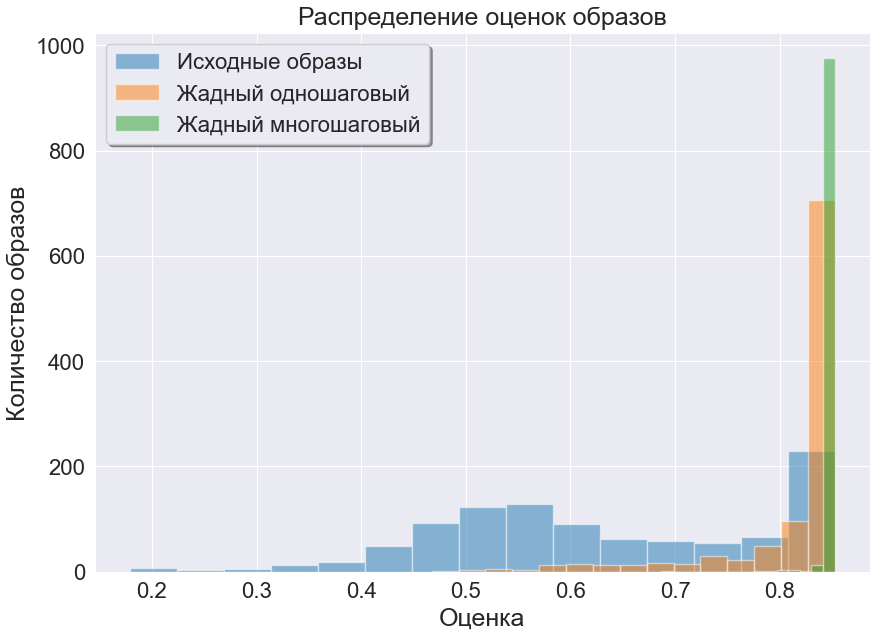
\includegraphics[scale = 0.7]{../figures/greedy_at_least_5_subset1000.png}
				
				Катастрофически долго работает, но хорошие результаты
				
			\subsection{Непрерывный подход}
			
			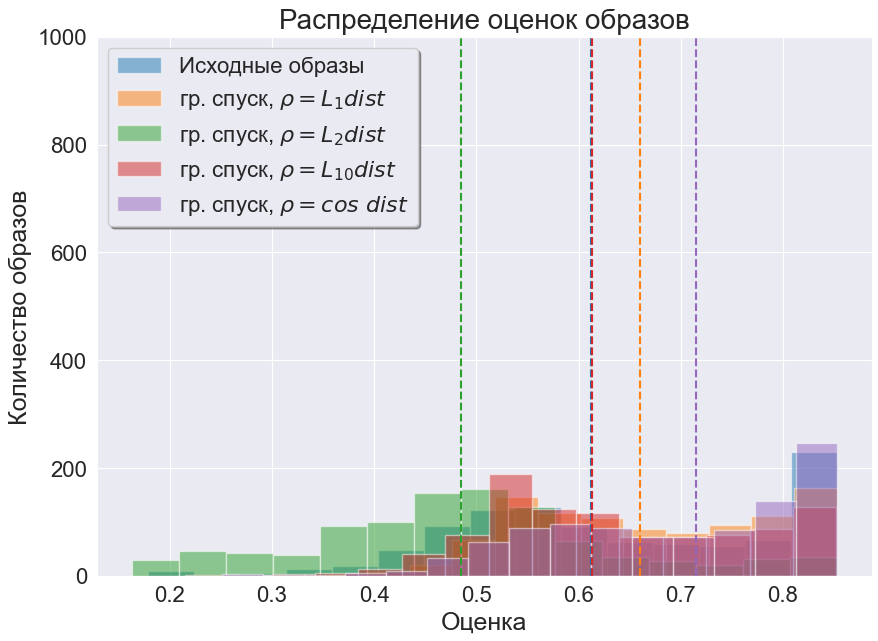
\includegraphics[scale = 0.7]{../figures/backprop_at_least_5_subset1000.png}
				
			как и предполагалось работает не очень 
			
			сильно зависит от выбора нормы, который можно осуществить только перебором и эмпирическими предположениями
			
			долго работает
			
			\subsection{Генерация скрытых представлений}

					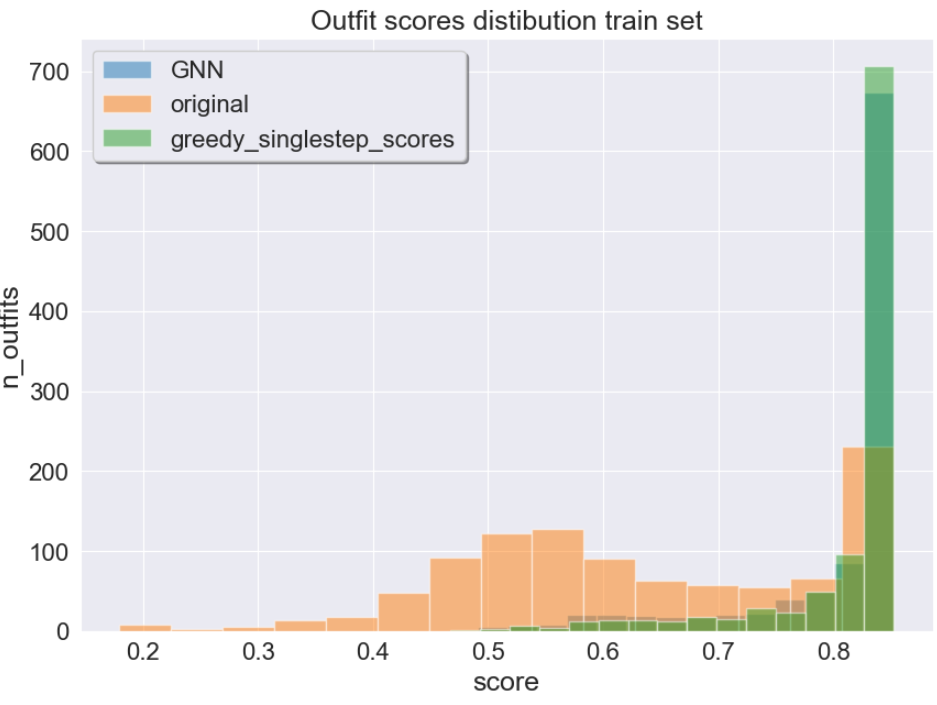
\includegraphics[scale = 0.7]{../figures/GNN_at_least_5_subset1000_train.png}
					

					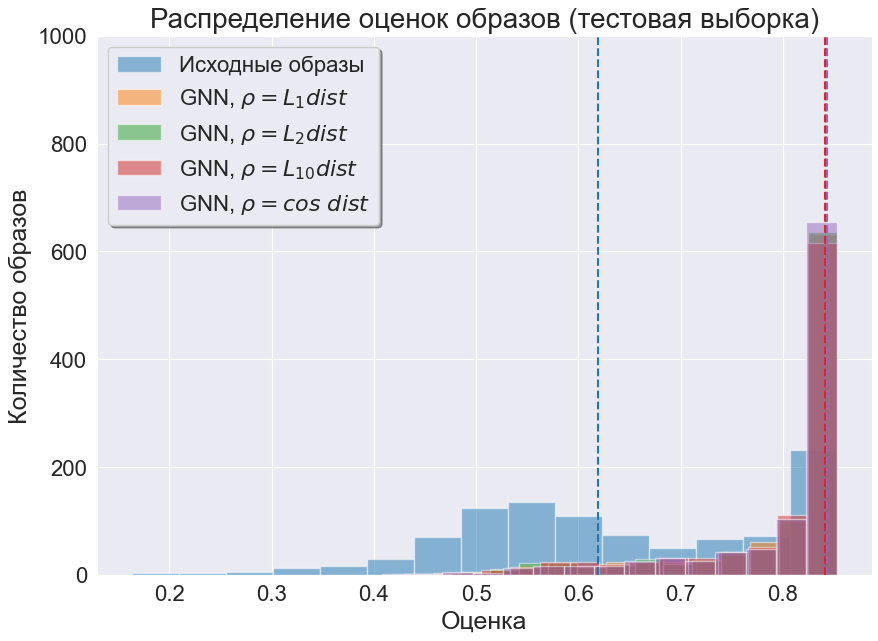
\includegraphics[scale = 0.7]{../figures/GNN_at_least_5_subset1000_test.png}
										
					Работает почти как одношаговый жадник, но быстрее на 2 порядка, что дает возможность применять на практике
					
					
					
					
			
			
			
			
			
			
			
	\bibliographystyle{plain}
	\bibliography{references}
			
	 
\end{document}